\chapter{Choice Poetics}

\label{ch:choice-poetics}

The aim of this chapter is twofold---first, to establish a framework for talking clearly and precisely about choices and their outcomes, and second, to introduce a method for analyzing choices based on how they relate to player goals.
%
Choice poetics should be able to address questions like: ``What is it about a choice that makes some players feel regret after picking a particular option?''
%
This chapter attempts to establish terminology and formal perspectives that can be used to talk about choices, but it's far from a ``complete'' theory of choice poetics: it only deals with explicit, discrete choices, for example.
%
Some parts of the theory are more developed (those that supported and were influenced by the development of \dunyazad/), but the ideas here are just the beginning of an in-depth study of narrative choices.


Note that here I define ``poetics'' broadly as the compliment of hermeneutics: if hermeneutics is the study of the meaning of a text, poetics can be understood as the study of its non-meaning-related qualities, such as the emotions or themes it evokes.
%
Poetics deals with the feelings that a player has before, during, and after making a choice, including simple feelings like the impression that a choice is difficult to make, but also complex feelings like regret.
%
It is also concerned with how these feelings help a work express themes or otherwise enhance the player's experience of a narrative, although the work presented here focuses mainly on the specifics of how choice structures engender feelings in the players who experience them.


\section{Inspirations}

\Cref{ch:related-work} contains a full review of literature related to choice poetics, but some of the most relevant sources are worth reiterating here.
%
While choice poetics clearly has roots in the work of Aristotle \citep{Aristotle1917} (and more recent narrative formalists like Freytag \citep{Freytag1894} and Barthes \citep{Barthes1975}, to name only a few) choice poetics is also inspired by investigations into the psychology of both reading and decisions.
%
In the first camp, psychologists have studied specific narrative effects such as transportation \citep{Green2000}, surprise \citep{Iran-Nejad1987}, and identification \citep{Oatley1995}.
%
In the second camp, researchers have studied how things like framing \citep{Tversky1981,Tversky1993}, and personality \citep{Schwartz2002} affect decisions and preferences.


Including craft wisdom from places like the Choice of Games development blog \citep{ChoiceOfGamesGameDesignCategory}, existing sources already contain a lot of information about how narrative choices function.
%
However, much of it is focused on either linear narratives or real-world choices, and the resources that do explicitly deal with narrative choices lack a solid theoretical foundation.
%
Some of the work of this chapter is therefore synthesizing this existing information into a theory concerned primarily with discrete, explicit choices in narrative contexts.


\section{Modes of Engagement}


In developing a theory of choice poetics, one must respect the lessons of the development of traditional poetics.
%
In particular, modern scholars have largely rejected ``objective'' narrative analysis and concluded that the experience of the individual reader must be taken into account.
%
Unlike Aristotle, who stated authoritatively what was good and bad about this drama or that, modern narrative scholars will analyze a work from a particular perspective, without claiming that this perspective is universal, perhaps performing a feminist or Marxist reading of a novel to see what insights a particular lens has to offer about the work.


Choice poetics must also respect the perspective of the reader, but it is in a slightly different position, as its readers are also players.
%
Insofar as the narrative that contains choices is experienced through the fabric of a game, the reader/players (henceforth players) are stepping into the magic circle of the game \citep{Huizinga1949} and intentionally taking on certain attitudes.
%
A narrative experienced within the framework of a game thus implicitly biases the attitudes of its readers, for example by setting up a score counter which players can try to maximize.
%
Counter-play is of course possible and important, but even counter-play is influenced by the rules of the game by virtue of being set against them.
%
The formal structures of the game rules that accompany a narrative-with-choices thus allow the theoretician to make an educated guess about the attitudes of players interacting with a piece.


There are still a range of attitudes that players can take on, however, and some understanding of this range is important before any analysis of choices in a narrative.
%
This range of attitudes has to some degree been studied by others interested in player types, although such studies are mostly focused on games without regard to narrative.
%
From simple binary ``casual/hardcore'' distinctions to more complex typologies such as Bartle's ``achievers,'' ``explorers,'' ``socializers,'' and ``killers,'' player type classifications to some degree incorporate notions of player intent or attitude \citep{Bartle1996}.
%
However, player type classifications also focus on player actions or approaches within the game, for example a distinction between those who enjoy stealth or direct combat more.
%
These player content preferences are as important as any other player preferences when it comes to how players approach choices, but they're less important than player motivations, which establish entire contexts within which preferences can be expressed.
%
For example, if one's motivation to play is a desire to act out a role, one's preferences might be expressed in terms of the kind of role one is trying to act out.
%
If one's motivation to play is to score points, on the other hand, preferences might be expressed in terms of different strategies for doing so.


The idea of ``modes of engagement'' captures these different player motivations.
%
Modes of engagement are different ways in which a player can approach a game.\footnote{%
Note that the idea of modes of engagement is not unique to games: different audience approaches have been acknowledged as important in areas such as education and music composition \citep{Langer1995,Brown2001}.}
%
At this point it is important to note that modes of engagement are neither exclusive nor permanent: players often engage in several modes at once (to varying degrees) and may change their modes of engagement during the course of play.
%
The modes of engagement presented here are also not intended to be comprehensive: these are some of the most common modes, but others may be possible and even the norm for certain games.
%
All of that notwithstanding, consideration of the mode(s) of engagement that players bring to a work is the first step in analyzing the choice poetics of a work.


This can take the form of assuming a particular mode: much as one can perform a feminist reading of a novel, one could perform a power-playing playthrough of a game.
%
This could also take the form of analyzing the game itself to determine which mode(s) of engagement it encourages and rewards.
%
It could even take the form of a qualitative study of actual players, to determine which mode(s) of engagement they are employing.
%
In any case, an analysis of choice poetics that does not consider modes of engagement is incomplete.


\Cref{tab:modes-of-engagement} lists some of the most common modes of engagement, and gives examples of decisions that employ them.
%
The last column references Nick Yee's work on motivations for play in massively-multiplayer online role-playing games as a comparison \citep{Yee2006}.
%
The grouping of Yee's motivation components into these modes of engagement has to do with a difference in focus: Yee is focused primarily on aspects of play, including a strong focus on online social interaction, whereas choice poetics is interested primarily in single-player offline engagement with an emphasis on narrative.
%
For example, Yee makes fine distinctions between different motivations grouped into the ``power play'' category here, but from a choice poetics perspective, whether someone is trying to maximize score or compete with an opponent doesn't matter, because both motivations are equally orthogonal to the narrative, and thus they have a similar effect on the player's experience of the narrative.


\begin{table}[!p]
\begingroup
\renewcommand*{\arraystretch}{1.5}
\begin{tabular}{p{5em}p{10em}p{10em}p{6.9em}}
\toprule
\textbf{Mode} & \textbf{Decision Process} & \textbf{Example} & \textbf{\citep{Yee2006}} \\
\midrule
\textbf{Avatar Play} & Decide as if you were in the character's situation. & When picking a pet, pick the cat because you like cats. & Role-Playing, Customization, Escapism \\
\textbf{Role Play} & Decide in order to act out a persona. & Choose the wizard character class because you want to play a shy, bookish person. & Role-Playing, Customization, Escapism \\
\textbf{Power Play} & Choose options that advance game metrics like score, beating other players, or quick completion. & Sacrifice an ally to obtain a powerful item because it helps you beat the game more quickly. & Advancement, Mechanics, Competition, Teamwork \\
\textbf{Explora-tory Play} & Choose options to see what will happen. & Turn away from the path of your quest to explore the world. & Discovery \\
\textbf{Social Play} & In a multiplayer situation, choose options because of social considerations. & Turn down a high-level quest in order to accompany your friend on a lower-level quest. & Socializing, \newline Relationship \\
\textbf{Analyti-cal Play} & Make decisions in order to analyze the work. & Repeatedly load a saved game to explore every possibility at a choice. & \emph{none} \\
\textbf{Critical Play} & Make decisions as performance to deconstruct or criticize a work. & Drive your character into poverty in order to demonstrate a game's biased depiction of poor people. & \emph{none} \\
\bottomrule
\end{tabular}
\endgroup
\caption[Modes of engagement]{Some common modes of engagement.}
\label{tab:modes-of-engagement}
\end{table}

Although modes of engagement are important to choice poetics, in my work with \dunyazad/ I have not given them great attention: \dunyazad/ encourages avatar play and all of its evaluations assume that players will engage primarily in this mode.
%
Extending \dunyazad/ to support power play and role play better, and to account for these possible approaches when evaluating choices, would be a very interesting line of future work.
%
Developing \dunyazad/ in that direction would allow it to be used as a tool to study modes of engagement in more detail.


\section{Dimensions of Player Experience}

When using choice poetics to analyze a narrative or even just a single choice, one must consider the range of expressiveness of narrative choices.
%
Aristotle devoted much of his analysis of emotion in \work{Poetics} to tragedy and the heroic epic as these were traditional forms in his day, but the full range of poetic effects is very broad, and includes both momentary impressions such as a single phrase that provokes disgust, and overall feelings, such as sympathy for a tragic figure.
%
To some degree, more complex effects depend on simpler ones, for example when an overall experience of sympathy depends on many individual positive evaluations of a character, along with negative reactions to bad things that happen to that character.
%
Of course, once choices are involved, the repertoire of effects is expanded, and it's important to have some understanding of what poetic effects a choice can possibly have.
%
Although no summary of possible poetic effects could hope to be complete, I have tried to list here a collection of important high-level aspects of a narrative experience that are strongly influenced by choice structures, including some which I believe are unique to narratives that contain choices.


\begin{table}[!p]
\begingroup
\renewcommand*{\arraystretch}{1.5}
\begin{tabular}{p{5.5em}p{14em}p{13.5em}}
\toprule
\textbf{Dimension} & \textbf{Description} & \textbf{Potentially Supported By} \\
\midrule
\textbf{Immersion} & The degree to which the player's attention is focused exclusively on the game. & Outcomes that are believable given options; option coverage of desired actions. \\
\textbf{Identifica-tion} & How comfortable the player feels in the role they play as their avatar. & Options that support player self-expression. \\
\textbf{Transpor-tation} & The degree to which a player thinks in terms of the game world rather than the real world. & Choices which force the player to reason from a character's point of view. \\
\textbf{Agency} & Alignment of player goals with game affordances. & Transparent choices where outcomes align with player goals.\\
\textbf{Influence} & Degree to which the player feels they influence in-game events (even if they do not control them). & Choices where outcomes are divergent and impactful. \\
\textbf{Autonomy} & The player's ability to choose and pursue a variety of goals at their own discretion. & Choices between goals rather than between methods of pursuing a fixed goal; non-exclusive outcomes. \\
\textbf{Responsi-bility} & Player feelings of responsibility for the actions of their avatar. & A mix of intentional outcomes that are good for and bad for other game characters. \\
\textbf{Regret} & Player feelings of regret for an in-game decision. & Negative outcomes that result from tempting options but which are still believable. \\
\bottomrule
\end{tabular}
\endgroup
\caption[Dimensions of player experience]{Some aspects of player experience that are influenced by choice poetics, along with some hypotheses about what kinds of choices might support them.}
\label{tab:dimensions-of-experience}
\end{table}

\Cref{tab:dimensions-of-experience} provides a brief overview of these important dimensions of player experience.
%
Except for identification, transportation, and immersion, each of these possible poetic qualities are unique to interactive narratives: without choices, they simply aren't possible.
%
Because of this, figuring out how choice structures contribute to these effects 
is an important task for choice poetics.
%
Of course, some of these effects, like agency, have already been extensively studied, often in broader contexts than just choice-based interactive narrative.
%
But it will still be important to understand how choice structures specifically contribute to these poetic qualities.
%
What follows is a preliminary analysis of each quality, based on craft wisdom and existing studies of games and real-world choices.

\begin{itemize}
\item \textbf{Immersion}---There are several different phenomena that the word immersion can refer to in games, including sensory immersion, mechanical immersion, and narrative immersion (see \citep{Ermi2005}).
%
Narrative choices of the kind studied here bear most on narrative immersion, although they could also be a source of mechanical immersion in some cases.
%
Immersion goes hand-in-hand with effects like identification and transportation.
%
Although counting immersion as a poetic quality discounts the role of the reader to some degree, immersion isn't independent of the structure of a narrative either.
%
In particular, it is possible for a narrative (choice-based or otherwise) to disrupt player engagement when it contains contradictions or otherwise complicates the reader's ability to understand it (see e.g., \citep{Douglas2001}).
%
This is particularly relevant when choices become involved, as they can easily become a source of frustration, either because the player wants to take an action which isn't provided as an option, or because the player views an outcome as inconsistent with the option that led to it.


\item \textbf{Identification}---Identification in traditional narrative is a key property and is heavily influenced by the actions and attitudes of characters (see e.g., \citep{Feilitzen1975,Oatley1995}).
%
In narratives that include choices, the player usually has some control over the actions of one or more character(s), although this control is often incomplete, especially when it comes to attitudes rather than actions.
%
This degree of control can enable a different type of identification in which the player actually assumes the psychological perspective of a character, as opposed to viewing them as a role model (see \citep{Klimmt2009}).
%
Choices could have a big impact on identification if they fail to include options which the player believes are reasonable and which correspond to the choice that the player would be most comfortable with in a given situation, simply because such a situation is an explicit manifestation of a difference between the player and the character (see e.g., \citep{Busselle2009}'s discussion of identification in linear narratives).
%
For example, if the player is a pacifist, but there are never options for negotiating with enemies or otherwise resolving conflicts peacefully, one would expect identification to be hindered.
%
This is complicated by role-playing, however: there is no reason that a player who is a pacifist in real life cannot enjoy the opportunity to play a bloodthirsty character in a game.


\item \textbf{Transportation}---Transportation is the re-centering of a player's perspective from the real world into a fictional world, and is closely linked with narrative immersion (see \citep{Green2000,Green2004}).
%
Although the original research on transportation focused on linear narratives (both textual and visual), a similar phenomenon called presence has been studied in interactive contexts \citep{Witmer1998}.
%
Unlike immersion, transportation is exclusive to contexts that involve fictional worlds.
%
Transportation is also to some degree linked to identification, as when one identifies with a character it becomes easier to project oneself into that character's world (see \citep{Busselle2009} on this point).
%
Again, the believability and completeness of options and outcomes is important when choices come into the picture.
%
In particular, feelings of control and an ability to successfully predict developments have been implicated as contributing to presence (see \citep{Witmer1998}).

\item \textbf{Agency}---Agency has been a core focus of games studies as a feeling uniquely enabled by interactive media (see e.g., \citep{Murray1997,Mateas2001,WardripFruin2009,Mason2013}).
%
The feeling of empowerment that results from being able to achieve one's goals contributes to agency, and an alignment of player goals with player-influenced outcomes is a powerful formula for agency \citep{Mateas2001}.
%
Obviously, such an alignment relates intimately to choice structures, as choice structures establish which outcomes can be influenced by the player and also help set player expectations as to their goals.
%
Given this, opaque choices---where the player is not able to foresee consequences given the setup and options---may decrease agency, because even if an outcome advances player goals, the player may not feel responsible for their success.
%
Additionally, choices where outcomes are tangential to a player's goals can frustrate agency: if you're told to save the princess but then given only choices about which commodities to buy or sell, your ability to proactively pursue your goal has been stifled.


\item \textbf{Influence}---If diegetic agency is an ability to proactively exert control over the story world (see \citep{Mason2013}) then influence is half of that: players' feelings of being influential in the narrative world.
%
Influence is important because fantasies of being powerful are one of the pleasures of both traditional and interactive narratives (see e.g. \citep{Olson2008}).
%
While the experience of agency also requires that players are able to use their influence \emph{proactively} (they must have enough information to make informed decisions, for example), there are plenty of games where the player characters are \emph{influential} but players cannot freely exercise this power to do whatever they choose.
%
For example, a game like \work{Final Fantasy} \citep{FinalFantasy} fully supports player fantasies of being heroic and influential, and if the player makes a mistake this role can be jeopardized, but the protagonists do not have any capacity to control the outcome of their story beyond fulfilling (or failing to fulfill) their fixed destiny.
%
Such a game does not offer players the pleasures of diegetic agency that are uniquely afforded by an interactive format, but it may still offer the pleasure of a power fantasy (a pleasure that is common to both interactive and traditional narratives).
%
Interactivity takes such power fantasies one step further by making them participatory: even when denied agency and thus unable to decide how their character's influence is applied, players are responsible for their character's achievements by virtue of ``pulling the trigger:'' without their input the story cannot move forward, even if that input is a simple ``yes'' or ``no.''
%
Of course, the choices that a player has can serve to advance or undermine this feeling of influence, especially when, for example, a player re-plays to explore multiple paths in a narrative and finds that nothing changes.
%
Divergent outcomes which matter within the story world are critical for maintaining a sense of influence across multiple playthroughs, although a mere suggestion of such can be sufficient when players do not re-play.
%
Important blind choices (where the player must pick an option knowing that the choice will be momentous but uncertain about the exact effects) are a common source of narrative tension which makes players feel influential without giving them a real sense of agency.


\item \textbf{Autonomy}---Autonomy is another relative of agency and influence, and can be summarized as the player's ability to choose and pursue their own goals within a game (see e.g., \citep{Ryan2006}).
%
Some amount of active influence is required to have autonomy, but whereas influence is concerned with outcomes, autonomy is concerned with goals.
%
Autonomy is also distinct from agency: when a game sets up nicely-balanced formal and material affordances, agency can be experienced even if autonomy is absent, as in a game like \work{Quake}.
%
The converse is also possible: an overabundance of autonomy can leave players uncertain about what to do, undermining feelings of agency.
%
A game that supports player autonomy provides a play-space within which players can choose their own goals.
%
To the extent that a narrative-focused game can provide this, it will appear more as a space for player-created stories than a fixed story that affords the player some choice.
%
Games like \work{Sim City} \citep{SimCity} and \work{The Sims} \citep{TheSims} provide play spaces within which players can create their own narratives, and this is achieved by offering non-explicit non-discrete choices which give the player a huge amount of options.
%
A lesser degree of autonomy can be present in more linear narratives when the player has choices which affect the goals and priorities of characters within the story.


\item \textbf{Responsibility}---A feeling of responsibility for one's own actions (as distinct from empathizing with a character who feels the burden of responsibility) is something uniquely afforded by interactive narratives (see e.g. \citep{Murphy2013}).
%
Choice structures are key to creating this, and there are several conditions for enabling responsibility.
%
First, the player must be given moral agency within the story world, which means that different outcomes at a choice must have consequences which have morally distinct outcomes.
%
Second, the player must be willing to take responsibility for their actions, and this can be impeded when they feel that the outcomes of their actions were unforeseeable or otherwise out of their control (of course, the feeling of a player who mentally justifies their lack of culpability for an in-game consequence is also an interesting poetic effect).
%
Note that this direct player-responsibility is different from role-played responsibility: it's possible for a player to role-play responsibility even when the actions they are assuming responsibility for were completely outside their control.
%
An example of responsibility (or the shirking thereof) as a poetic effect happens in the game Portal \citep{Portal}, when the player is forced to incinerate their companion cube in order to progress within the game.
%
The complex emotions that arise at that moment are the result of a forced choice between two bad outcomes (being unable to progress and incinerating the companion cube\footnote{Note that this analysis makes assumptions about the player's goals and feelings: some player communities see the companion cube itself as an obstacle worthy of hatred rather than a helper who deserves pity, and so view this choice in a very different light.}), and the moment has emotional resonance later in the game when the player has the opportunity to destroy GLaDOS---the agent which forced the decision upon the player---using similar means.


  \item \textbf{Regret}---Like responsibility, the capacity to make players feel regret is mostly unique to interactive narrative (see \citep{Frome2006,Zagal2009}).
%
Again, in linear narrative it is possible to sympathize and empathize with a character who is feeling regret within the story, but that's a different feeling than personal regret for one's own actions (a book or film might also cause one to revisit a personal regret, but this again is different from being the cause of that regret).
%
As with responsibility, making a player feel regret is quite delicate: the player not only has to achieve some level of transportation and identification, but the choices involved must be structured to resist the player's natural tendency to reassign blame.
%
With a negative emotion like regret, the basic psychological mechanisms of denial are the brain's first line of defence, and so naturally the narrative and choices leading up to a moment of regret will be scrutinized for interpretations that leave the player blameless.
%
In particular, if the player can convince themselves that the game forced them to make a choice that led to a negative outcome, or that the outcome was unforeseeable given the option that led to it, they can often avoid regret.
%
Of course, this process of denial is an interesting poetic effect in its own right, and in some cases is exactly what an author wants (perhaps so they can later force the player to re-examine their denial and admit blame, thus experiencing even more poignant regret).
%
A game like The Walking Dead \citep{TheWalkingDead} forces the player to make many difficult decisions between options with divergent but uniformly negative consequences, and this pattern engenders feelings of desperation and regret.

\end{itemize}


Each of these topics could be (and some of them have already been) the topic of dedicated research.
%
However, they are presented here merely to demonstrate how much there is to learn about choice poetics---\dunyazad/ as a system does not focus on any of these, but rather attempts to get at some simpler phenomena, such as what makes an individual choice obvious, or what is required for a choice to be seen as a dilemma.
%
Patterns of choices with specific properties such as obviousness or unexpectedness of outcomes come together to produce higher-level poetic effects like those described here, and a better understanding of these low-level effects is required in order to aim at higher-level effects.
%
The poetic details that \dunyazad/ actually operationalizes are based on player goals, and the perceived relevance of options and outcomes to them.
%
As \dunyazad/ only reasons about one choice at a time, its logic effectively comprises an analysis technique for examining the basic poetic properties of an individual choice.
%
The next section describes this technique and how a human would apply it to an individual choice within an interactive narrative, while \cref{ch:dunyazad} describes how \dunyazad/ operationalizes this theory, and \cref{ch:option-results,ch:outcome-results} describe how results from two experiments using \dunyazad/ have informed both the theory and the system.

\section{Goal-Based Choice Analysis}

\label{sec:goal-based-choice-analysis}

When authoring a choice or attempting to understand an existing choice, the method of analysis presented here can help tease out how a choice might be perceived by players.
%
This method is grounded in player goals: it views each option and outcome through the lens of what the player wants, and then tries to synthesize this information to understand how an entire choice is perceived.
%
\Cref{fig:choice-analysis-method} gives an overview of the technique described in this section, which consists of seven steps.
%
The basic idea is to carefully break down how the options and outcomes relate to player goals, attempting to consider as many details as possible, and then synthesize those detailed assessments back into high-level assessments of the choice as a whole.
%
The next section describes the methodology used to come up with this analysis method, while the following section describes in detail how a discrete, explicit choice is represented for this analysis, and the seven analysis steps are described in the remaining sections.


\begin{figure}[!p]
\centering
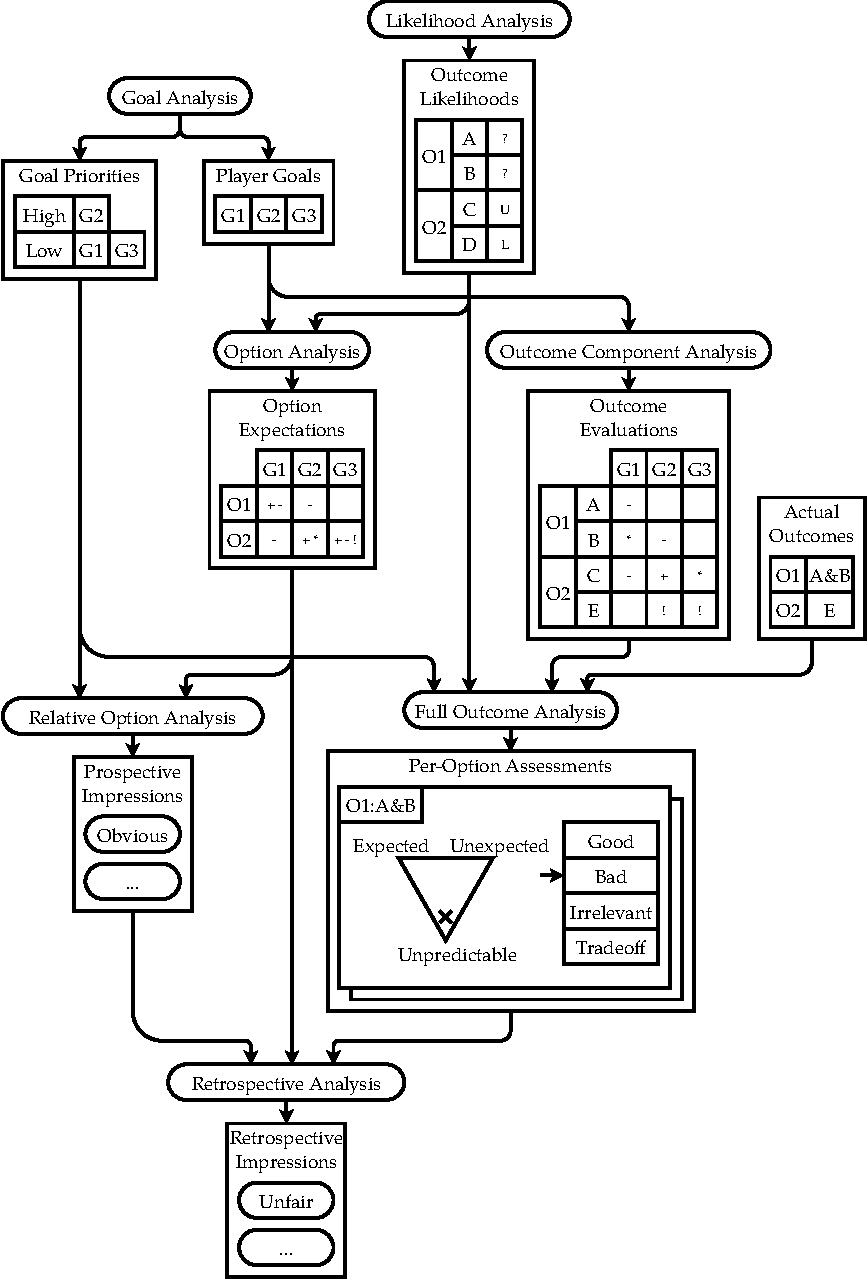
\includegraphics[height=0.92\textheight]{fig/analysis-method-crop.pdf}
\caption[Choice analysis flowchart]{Goal-based choice analysis for a single choice---an overview of the different steps and the information produced.}
\label{fig:choice-analysis-method}
\end{figure}

\subsection{Methodology}

It is worth reiterating the process used for the creation of this analysis technique.
%
A traditional approach might start with a critic observing regular patterns in choices, and invent a rudimentary framework for recognizing these.
%
Such a critic might then attempt to apply this nascent analysis technique to choices in a few well-known games, and then refine it based on these results, continuing this cycle until the method was deemed satisfactory.


Instead, this technique has been developed with reference to the generative system described in \cref{ch:dunyazad}.
%
Using the desire to generate poetic choices as motivation, the question ``What aspects of a choice need to be understood by the system?'' was posed, and a combination of existing systems, craft advice, and theories of both psychology and narrative were consulted to come up with a preliminary answer (see \cref{ch:related-work}; e.g., \citep{Mott2006,ChoiceOfGamesChoiceRules,Shepperd2002,WardripFruin2009}).
%
This initial approach pointed to several important factors: player goals, players' evaluations of the relationship between outcomes and these goals, and things like expectations and likelihoods.
%
These are factors that have been used by existing systems, are the subject of craft advice, appear as variables in psychological studies of decision-making, and are components of theories of interactive narrative.


After identifying these factors as important, the next step was a technical one: using these factors as underlying variables, an answer-set programming framework for representing choices was developed (see \cref{ch:dunyazad}).
%
Technical development proceeded until the system could manipulate these variables and generate rudimentary choices.
%
Of course, the choices it generated at first were flawed, and development of both the theory and the system proceeded through several rounds of revision, using flawed results from the system to motivate elaborations of the theory.


The end product of this methodology for theory development looks a bit different than the results of the traditional approach.
%
For one thing, it is more detailed: because the theory was operationalized early in its development, it naturally contains enough specifics to be evaluated mechanically without necessarily depending on human `common sense' to apply complex criteria.\footnote{%
Of course, humans are still better at applying even the specific criteria of this analysis method, for example when comparing the impact of outcomes they can discern many differences that the generative system cannot.
%
As seen in the following chapters, there is no substitute for humans when it comes to understanding how humans feel; the technique developed here only allows \dunyazad/ to guess correctly in \emph{some} situations, although refinements suggested by experimental results may been able to improve things.
}
%
Another result of the system's unique development path is modularity: each step of the analysis is designed to move from one set of evaluations to another without depending directly on the details of any other step.
%
This modularity is not necessarily beneficial for the resulting analysis technique as a technique, but it does help when attempting to diagnose problems with the system (and thus also with the theory).
%
The separation of modules also allows the theory to be subject to incremental change: an improved method for a specific step could be proposed without needing to overhaul the entire approach.



\subsection{Choice Representation}

\label{sec:cp-choice-representation}

This method is developed primarily for the analysis of explicit discrete choices, and for these choices a detailed breakdown of their structure is possible.
%
\Cref{fig:choice-anatomy} shows how a choice (in this case one generated by \dunyazad/) can be broken down into framing, options, and outcomes.
%
Note that it can be useful to further break down outcomes into individual \emph{outcome components}: individual changes that result from choosing an option which are significant on their own.
%
By doing so, the impact of each outcome component on individual player goals can be analyzed separately, which helps understand outcomes that involve complex trade-offs between multiple goals.
%
Not shown in \cref{fig:choice-anatomy} are unrealized outcome components which nevertheless factor into the choice analysis.
%
For example, if the player were unlucky, the third option might not have resulted in the bandits calming down, and one could even imagine a situation where the bandits might turn on the player.
%
Separate analysis of potential outcome components, such as ``the bandits calm down'' or ``the bandits become angry with the player'' can be used to examine in detail how each option differs from alternatives, even when some outcome components are exclusive of or linked to each other.
%
It's also the case that understanding what the player thinks \emph{might} happen as a result of choosing a given option is just as important as recognizing what does happen as the story unfolds.
%
Finally, this idea of potential outcome components can also help analyze cases where a system is nondeterministic, and the outcomes of a choice vary between playthroughs.
%
Each part of a choice is subject to scrutiny using the methodology presented here, and having precise language to talk about these choice components is necessary for detailed analysis.

\begin{figure}[!p]
\centering
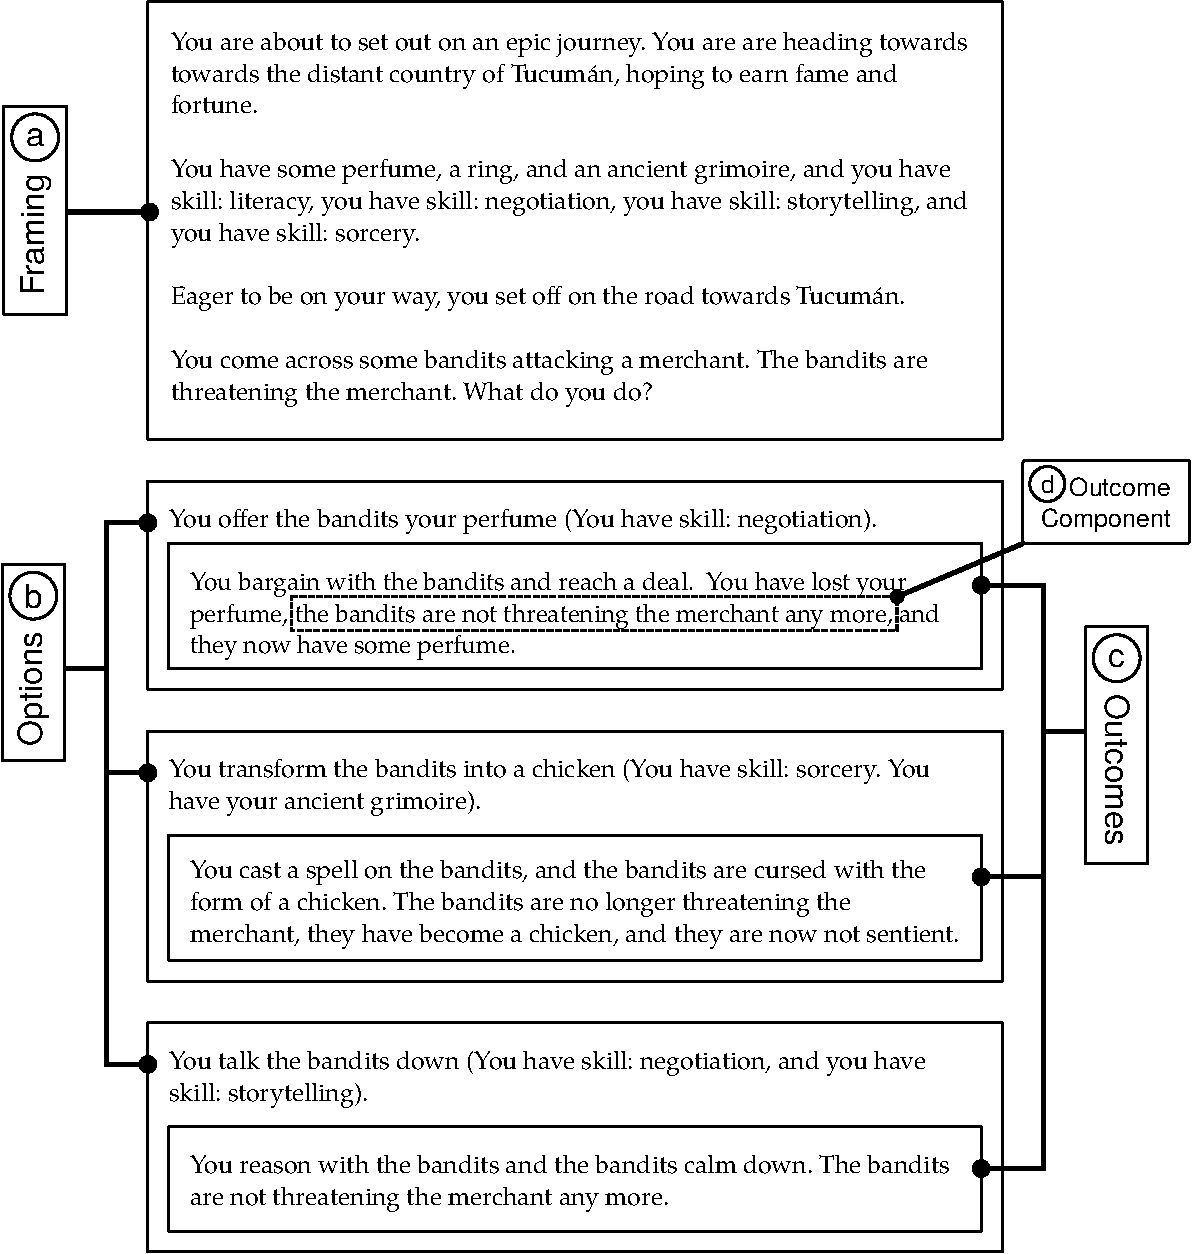
\includegraphics[width=\textwidth]{fig/choice-anatomy-crop.pdf}
\caption[Anatomy of a choice]{%
\setstretch{1.1} % Else the \encircles would stretch only some of the lines
\addtolength{\baselineskip}{0pt plus 1pt minus 1pt}
Anatomy of a choice (using one generated by \dunyazad/).
%
\encircle{a}~Framing---sets up the narrative situation at the choice.
%
\encircle{b}~Options---discrete options available to the player.
%
\encircle{c}~Outcomes---Not initially visible to the player, but revealed after a decision is made.
%
Each option has a single corresponding outcome.
%
\encircle{d}~Outcome components---Individually significant changes that result from picking a particular option.}
\label{fig:choice-anatomy}
\end{figure}


\subsection{Goal Analysis}

\label{sec:cp-goal-analysis}

As already mentioned, poetic analysis of a choice depends on some understanding of the player's approach to the choice.
%
For goal-based choice analysis, this is taken into account by coming up with a list of player goals.
%
Depending on the objective of analysis, there are different ways to come up with this list.
%
One method is to simply list the goals that the analyst themselves would have when approaching the choice.
%
Another is to try to put oneself in the shoes of a particular type of player, perhaps according to one of the modes of engagement listed above.
%
This can be useful for an author trying to figure out how different types of players will perceive a choice: just come up with goal lists corresponding to each player type of interest and perform separate analyses using each list.


In any case, coming up with these lists should take into account not only the desires of the actual or imagined player, but also what aspects of the framing of the choice and previous content encourage which player goals.
%
Based on the options available at previous choices and the narrative content, games can not only encourage certain general modes of engagement, but can establish and encourage the pursuit of specific goals.
%
This encouragement itself often depends on a player's mode of engagement to function as intended, however.
%
For example, game rules directly establish goals for power gamers, but players who have a different mode of engagement may not care about those goals.


If an important goal is missing from the goal list, the entire analysis may be skewed, so it's important to consider the full set of probable player goals.
%
On the other hand, it's always possible to come back to the goal analysis if one realizes during a later step that there's an additional goal that might be relevant. 
%
This is not uncommon, as the particular set of options and outcomes at a choice  determines which goals are relevant.
%
However, part of the point of performing goal analysis before even considering the structure of the choice in question is to avoid bias.
%
This also means that the results of goal analysis can be re-used when analyzing multiple choices.
%
Of course, player goals may change over the course of a game, and this must be taken into account, but performing a full goal analysis from scratch for each individual choice is generally not necessary.


Besides just listing player goals, a goal analysis must give some notion of their relative priorities.
%
This can be as simple as sorting the goals into ``high'' and ``low'' priority tiers, but a more detailed representation of priorities can also be used.
%
This priority information is used when combining information about multiple options and outcomes during the relative option analysis and full outcome analysis steps.
%
Because goal priorities are even more volatile and difficult to estimate than goals themselves, sometimes it's simplest just to wait until the later analysis steps to consider goal priorities, as there will likely be only a few specific goals (those relevant to the choice in question) for which priorities actually affect the analysis.


\subsection{Likelihood Analysis}

\label{sec:cp-likelihood-analysis}

The second step of analysis is to figure out which potential outcome components are made to seem likely by the framing and option text of the choice, and assign each component a label of \lbl{likely}, \lbl{neutral}, or \lbl{unlikely}.
%
For each option, this step starts by identifying a set of outcome components that seem plausible, and then figuring out which of those are likely and unlikely.
%
The goal of this step is to identify outcome components that the player can \emph{presume} will result from each option, so if there are actually multiple conflicting likely scenarios (combinations of outcome components), only outcome components present in \emph{all} probably scenarios count as \lbl{likely}.
%
For example, if one option involves rolling a six-sided die, but the player has been given a prophecy that the result will be either a six or a one, then the outcome components associated with rolling a six and those associated with rolling a one are all \lbl{neutral} in this analysis, while outcome components associated with other rolls are \lbl{unlikely}. 
%
Any outcome component that's associated with both rolling a six and rolling a one would still be marked as \lbl{likely}: given the information the player has, they can assume that such an outcome component will happen if they choose to roll the die.


The outcome likelihoods produced by this step are used during option analysis in combination with the list of player goals from the goal analysis to figure out how each option portrays itself as affecting each goal.
%
\Cref{fig:choice-analysis-method} displays these assignments in the `Outcome Likelihoods' box: the choice has two options, `O1' and `O2,' and O1 suggests outcome components `A' and `B,' while O2 suggests outcome components `C' and `D.'
%
Components `A' and `B' are both \lbl{neutral} (indicated by a `?'), while component `C' is \lbl{unlikely} (a `U') and component `D' is \lbl{likely} (an `L').
%
Note that it's possible and even common for the same outcome component to be a plausible result of multiple options, although that situation is not shown in \cref{fig:choice-analysis-method}.


During this step, the actual outcomes of each option are irrelevant; what's important are the cues present in the framing and options that hint at what might happen if an option is elected.
%
This often includes a large body of implicit player knowledge that depends on player experience with a game: players who have played a game already (or even just games from the same genre) may build strong expectations from minimal cues.
%
Much like player goals, potential and likely outcomes from a player's perspective can be difficult to predict perfectly.
%
However, from a designer's perspective, each choice is usually explicitly crafted to present certain outcomes as most salient, and in that case, this step of analysis is mostly focused on double-checking the framing and options to ensure that they highlight the intended outcomes properly.


\subsection{Option Analysis}

\label{sec:cp-option-analysis}

Given the player goals and estimates of likely-seeming outcome components, option analysis proceeds by analyzing how each option seems likely to impact each goal, aggregating information across outcome components at each option.
%
First, all \emph{possible} outcome components are considered, to come up with an estimate of the goals that could possibly be impacted by each option.
%
These evaluations are \lbl{enables} and \lbl{threatens}---which goals each option might possibly advance, and which goals it might possibly impede.
%
In \cref{fig:choice-analysis-method} the `+' and `-' symbols in the `Option Expectations' box are these \lbl{enables} and \lbl{threatens} assignments.


Essentially, these \lbl{enables} and \lbl{threatens} evaluations are produced by considering the impact of each outcome component on each goal.
%
If any possible outcome component of an option could negatively impact a particular player goal, it is said that that option \lbl{threatens} that goal.
%
Likewise, if an outcome component can positively impact a goal, it is said that that option \lbl{enables} that goal.
%
It is possible and even common that an option both \lbl{enables} and \lbl{threatens} the same goal, and of course it's also possible that it neither \lbl{enables} nor \lbl{threatens} a particular goal (or even any goal at all).
%
For example, an option to ``attack the dragon'' presumably both \lbl{enables} and \lbl{threatens} the goal of preserving one's life, as both being killed and surviving are \emph{possible} outcome components (even if one seems more likely than the other).


Besides \emph{possible} impacts of each choice, option analysis is also concerned with \emph{likely} impacts.
%
Using the same procedure, but this time only considering \lbl{likely} outcome components, \lbl{advances} and \lbl{hinders} option expectations are assigned to each option/goal pairing (these are the `*' and `!' symbols in the `Option Expectations' box of \cref{fig:choice-analysis-method}).
%
In other words, when an option's \lbl{likely} outcome component positively impacts a goal, that option is said to \lbl{advance} that goal, and a similar negative impact results in a \lbl{hinders} label.
%
If it's not clear whether an option \lbl{advances} or \lbl{hinders} a goal (perhaps because of multiple conflicting outcome components), neither label should be assigned: the \lbl{enables} and \lbl{threatens} labels should already be present and serve to indicate the possible but uncertain outcome relative to that goal.
%
On the other hand, if contrary indicators are present but one is clearly stronger or much more likely than another, the label more strongly indicated can be assigned, but this should only be done if the player can safely assume that the goal will be affected as indicated, as that is the purpose of these labels.
%
Note that an \lbl{advances} label can only be present if there is an \lbl{enables} label, and similarly a \lbl{hinders} label requires the presence of a \lbl{threatens} label.
%
The combination of \lbl{enables}, \lbl{threatens}, and one of either \lbl{advances} or \lbl{hinders} is common, and indicates an option that will probably advance or hinder a goal but with some risk involved.
%
For example, the hypothetical ``attack the dragon'' option discussed above might not only \lbl{enable} and \lbl{threaten} the goal of self-preservation but also \lbl{hinder} it, if the player believes that being killed is a \lbl{likely} outcome component and that staying alive is not.


The separate analysis of all vs\@. \lbl{likely} outcome components and the four labels that result allow a wide range of choice structures to be accurately described in simple terms, especially when comparing labels assigned between one option and multiple goals.
%
The analysis of all possible outcome components for the \lbl{enables}/\lbl{threatens} labels captures a broad view of option/goal relationships while the \lbl{advances} and \lbl{hinders} labels based on only \lbl{likely} outcome components capture information about the perceived ``most likely scenario.''
%
Patterns across multiple goals (for example a ``tradeoff'' when one goal has an \lbl{advances} label while another has a \lbl{hinders} label at a particular option) are easily recognizable, and this is the basis for the relative option analysis step.


Remember that this step still makes no use of the actual outcomes of an option: it is just concerned with how the player views each option before making a decision.
%
It can also ignore the goal priorities because each goal is considered separately.
%
The option expectations produced by this step are used in the relative option analysis and retrospective analysis steps as a formal representation of how the player views each option.
%
During those analyses more fine-grained evaluations of player perceptions may be required on a case-by-case basis, but the \lbl{enables}/\lbl{threatens}/\lbl{advances}/\lbl{hinders} labels allow such complicated cases to quickly be separated from the simple cases.


\subsection{Relative Option Analysis}

\label{sec:cp-relative-option-analysis}

After producing option expectations for each goal/option pairing, a full-blown analysis of the choice from a pre-decision standpoint can be produced by comparing the options available.
%
A set of prospective impression labels can be used to identify common option structures, and choices that don't easily fit into a known category can be examined more closely.
%
This step uses not only the option expectations from the option analysis step, but also the goal priorities that were produced during goal analysis.


Certain common patterns of option expectations create well-understood prospective impressions.
%
For example, a dilemma has a specific feel, and several types of dilemma can be easily identified by comparing option expectations.
%
If there are exactly two options at a choice, each has overall negative impacts on high-priority player goals (and these impacts are roughly balanced), and each option negatively impacts a different set of goals, then the choice is a classic dilemma.
%
All of this information (besides the balance of impacts) is directly encoded in the goal analysis (priority information) and the option analysis (\lbl{hinders} labels) results, so classic dilemmas are easy to identify using this analysis method.
%
From a design standpoint, it's also easy to identify when an option isn't a classical dilemma and which aspects of that option would need to change to make it one.
%
Given the detailed language of choice analysis it's further possible to describe other kinds of dilemmas: a two-option choice with balanced positive outcomes, or a three-option choice that still has balanced outcomes, or even a tradeoff choice where each option has positive impacts on one of two goals and negative impacts on the other.
%
This is one of the benefits of a detailed analysis technique, in fact: developing the precise language necessary for describing choices formally establishes a framework within which variations on a common pattern can be identified and enumerated.


\begin{table}[!p]
\begingroup
\renewcommand*{\arraystretch}{1.5}
\begin{tabular}{p{4.5em}p{10em}p{18.5em}}
\toprule
\lbl{Label} & \textbf{Description} & \textbf{Criteria} \\
\midrule
\lbl{Depres-sing} & A choice where no matter which option you choose, there's a goal that's hindered . & Every option \lbl{hinders} at least one high-priority goal. No option should \lbl{enable} or \lbl{advance} any high-priority goals. \\
\lbl{Dilemma} & A difficult decision between two negative outcomes. (A particular kind of \lbl{depressing} choice.) & Exactly two options, each of which \lbl{hinders} one of two different high-priority player goals. The priorities of the goals and the severity of the consequences should be balanced and neither option should \lbl{enable} or \lbl{advance} any goals (even low-priority ones). \\
\lbl{Empower-ing} & A choice where every option has a positive impact. & Every option \lbl{advances} a player goal, and may \lbl{threaten} one or more goals but does not \lbl{hinder} any. \\
\lbl{Obvious} & A choice that has one option which is clearly better than the rest. & One option that \lbl{advances} a high-priority player goal without \lbl{hindering} any (although it may \lbl{threaten} some), while none of the rest of the options \lbl{enable} any high-priority goals, and each of them \lbl{threatens} some goal. \\
\lbl{Relaxed} & A choice that has no impact on any high-priority goals and where no goals are threatened. & There are no option expectations involving high-priority goals (positive or negative), and there are no \lbl{threatens} expectations (and thus no \lbl{hinders} expectations). \\
\lbl{Myster-ious} & A choice where there is no indication of which option is best or how the outcomes might affect things. & There are zero option expectations, including \lbl{enables} and \lbl{threatens} expectations. \\
%\textbf{Uncom-fortable} & A choice where the best option isn't very good, but it's better than the alternatives. & There's one option which is expected to \lbl{enable} an important player goal (but not to \lbl{advance} it), while every other option has some combination of \lbl{threatens} and \lbl{hinders} expectations. The enabling option also \lbl{threatens} and possibly \lbl{hinders} the goal that it \lbl{enables}. \\
\bottomrule
\end{tabular}
\endgroup
\caption[Prospective choice impressions]{Several different prospective impression labels, with formal criteria based on option expectations and goal priorities. Note: see \cref{sec:results-prospective-caveats} for a detailed discussion of some of these labels informed by experimental results.}
\label{tab:prospective-impressions}
\end{table}


\Cref{tab:prospective-impressions} gives an overview of some prospective impression labels and the criteria for applying them based on goal priorities and option expectations.
%
Note that the criteria are designed to be sufficient for applying the label, but not necessary---there are certainly some obvious choices which do not meet the strict criteria set out here, but from a design standpoint, if the criteria are met, a choice is almost certainly obvious (assuming also that the goal and outcome analyses are accurate of course).
%
The labels in \cref{tab:prospective-impressions} and their criteria were developed as part of \dunyazad/'s choice analysis component, and some of them (the \lbl{depressing}, \lbl{empowering}, \lbl{obvious}, and \lbl{relaxed} labels) were refined based on experimental results (see \cref{ch:option-results,ch:outcome-results}).


As a preview of those results, one caveat that applies to the \lbl{relaxed} label is that some people will always seek a best possible outcome when given a choice, and thus even at a choice among supposedly positive outcomes, options which appear to lead to \emph{relatively} worse outcomes may be seen as bad options \citep{Schwartz2002}.
%
See \cref{sec:results-prospective-caveats} for further discussion of some extra considerations for applying these labels.


The labels presented here give an idea of how players will feel when faced with this choice before they make a decision.
%
Classic dilemmas, for example, are stressful decisions which are difficult to make: they represent significant negative events and are a source of narrative tension (see \citep{Barber2007a}).
%
In linear narrative, dilemmas and their consequences are commonly used as low points in a story, and are themselves often a result of a character's previous poor decision, in effect serving as extended punishment: the character must not only suffer a negative consequence, but must also choose which consequence to accept, thereby being forced to reflect on their initial decision while agonizing about their present options.
%
Despite being negative moments, dilemmas can also serve as moments of clarity: when a character finally confronts the bad options available to them and makes a decision, this can mark the end of denial about their situation and ultimately the beginning of redemption.


In an interactive narrative, presenting the player with a dilemma can serve the same purposes: to accentuate an earlier mistake and punish the player, while perhaps also establishing a new goal of moving towards atonement.
%
A classic dilemma is a moment of heightened tension, and when a player is forced to make the decision it also represents a pause in the action, although a dilemma where the player has limited time to choose can also be used to accentuate feelings of urgency and haste (\work{The Walking Dead} makes effective use of both kinds of dilemmas \citep{TheWalkingDead}).
%
Additionally, when a player is confronted with a diegetic dilemma, any reasoning about which option is best is done from a point of view within the narrative, which may serve to heighten transportation.
%
At the same time, since diegetic dilemmas can force the player to make an important decision for their avatar and to ``think as'' their avatar, they may promote identification.


Dilemmas can be very fragile, however, because if the goals hindered by the two options are not well-balanced, the choice can become obvious (this impacted the experiments described in \cref{ch:option-results,ch:outcome-results}).
%
A dilemma may also force a player to re-evaluate their priorities, especially when the player goals involved relate to different modes of engagement.
%
For example, if one option hinders a player's ludic goal of becoming more powerful (without necessarily affecting a similar diegetic goal) while another hinders the diegetic goal of preserving the safety of their avatar's ally, many players may simply make a decision to prioritize one mode of engagement (avatar play or power play, in this example) over the other, and thus avoid the dilemma.
%
Of course, a choice like this that forces the player to decide between orthogonal goals can be used intentionally by an author to build divergent experiences for players who presumably prioritize different things.
%
Such a choice not only measures a player's priorities but also probably affects them: human cognitive biases related to self-consistency and rationalization mean (see e.g., \citep{Hall2012}) that once a player commits to a certain set of priorities they are likely to stick with that choice.


A label like \lbl{dilemma} can thus be unpacked into a rich understanding of the poetics of a choice.
%
Beyond assigning such well-understood labels, however, relative option analysis can also find choices which don't strictly conform to any labels, and analyze them on a case-by-case basis.
%
It is often useful to compare a specific choice structure to known structures and focus on the differences.
%
For example, a choice that meets all the criteria for being \lbl{obvious}, but where the best option also \lbl{hinders} a high-priority goal, could be compared to an \lbl{obvious} choice.
%
In this case, the relative merits of the goals \lbl{advanced} and \lbl{hindered} by the best option might mean that the decision is still straightforward, but even so the player may feel some reluctance that a normal \lbl{obvious} choice would not create.
%
Alternatively, because of the \lbl{hindered} goal and despite the \lbl{advanced} goal, an option which \lbl{threatens} some unimportant goal and has no other expectations might be more desirable than the `best' option if the player is risk-averse, creating a very different impression.
%
The relatively narrow labels presented here thus serve as anchor points for the analysis of more complex choices.
%
Of course, it's possible to establish many more clearly-defined labels than those presented in \cref{tab:prospective-impressions}, and doing so is a straightforward way to increase our understanding of choice poetics.


\subsection{Outcome Component Analysis}

\label{sec:cp-outcome-component-analysis}

While the results of relative option analysis give a sense of how a choice is perceived just before the player makes a decision, more work is necessary to understand how a player feels after experiencing an outcome.
%
This begins with outcome component analysis: Using the list of player goals and the actual outcome components at each option (as opposed to the potential components identified during likelihood analysis), a breakdown of the actual impact of each outcome component on each player goal is created (unlike the option analysis step, this step does not aggregate information across outcome components at each option, instead evaluating each outcome component/goal pairing individually).
%
Recall that the option analysis step already summarized how the framing and options of a choice indicated goals would be affected, but during this step, actual effects based on actual outcome components are considered instead of hypothetical effects based on potential outcome components.


An example of this distinction can be helpful: let's say the player has been flung off of a cliff and faces a choice between grabbing a nearby branch to save themselves or grabbing the outstretched hand of their avatar's only child, who is also falling.
%
As presented, the outcomes look grim: sacrifice any hope of saving one's child to save oneself, or catch one's child and at least suffer the same fate.
%
Assuming that the player can't reasonably expect some sort of miracle to save them (even given the full implications of genre conventions, etc.) both options are portrayed to have likely negative impacts on several player goals (assuming an avatar play mode of engagement).
%
But perhaps if the player chooses to grab their child, the actual outcome is that a freak gust of wind blows them both to safety, while if they choose to grab the branch, their child falls and dies.
%
This outcome component of being blown to safety would not appear during likelihood analysis and it would thus not be considered during option analysis, but as it is an actual outcome component, outcome component analysis would evaluate it (see outcome component `E' in \cref{fig:choice-analysis-method}).
%
The goal of outcome components is to analyze the valence of actual outcome components with respect to each player goal, including any components that weren't suggested by the framing and options of a choice.


The method is simple: for each outcome component that actually happens at each option (or when outcomes are non-deterministic, for each outcome component that could happen), estimate its impact on each player goal.
%
The `Outcome Evaluations' table in \cref{fig:choice-analysis-method} that results from outcome component analysis illustrates this, using `$\uparrow$', and `$\downarrow$' for minor positive and negative consequences, and `$\uparrow\uparrow$' and `$\downarrow\downarrow$' for major consequences respectively.
%
Of course, a finer gradation of consequences could be used if desired, and certainly should be employed on a case-by-case basis where specific consequences must be compared, but gross distinctions are often sufficient to analyze straightforward choice structures.


Note that even though the outcome component `C' of outcome `U2' does not actually occur according to the `Actual Outcomes' table, it is still analyzed in this example, perhaps because it might occur depending on the circumstances.
%
In contrast, the suggested outcome component `D' of option `O2' does not appear in the analysis of `O2's outcome `U2,' presumably because although implied as a possibility, it will never actually occur.
%
Outcome component `E' is the opposite: it was not implied, but does occur, and so must be analyzed.
%
There are thus several categories of outcome components: \emph{suggested} components that are hinted at by the framing and option text of a choice, but which may or may not even be possible, \emph{potential} components which are possibilities given a specific decision, \emph{actual} components which actually happen in a given play-through, and \emph{unrealized} components which could have happened given a particular decision but did not.
%
In the example analysis from \cref{fig:choice-analysis-method}, outcome components `A,' `B,' and `C' are both suggested and potential, while component `D' is only suggested.
%
Meanwhile, components `A,' `B,' and `E' are actual, while `C' is unrealized; note that component `E' is not a suggested component.


Depending on the interactive narrative, complex rules may exist that establish what configurations of actual outcome components out of the set of potential outcome components are valid, and the player may or may not be aware of these rules.
%
If analysis is being conducted without a specific playthrough in mind, then in latter stages the different possible combinations of potential outcome components will have to be considered separately, as each may give rise to a different player experience.
%
Of course, player experiences must already be separated based on which option is chosen, but this does add some complexity to the analysis.
%
In the rest of this chapter outcomes are assumed to be deterministic, as that is the case for choices generated by \dunyazad/, and it generally makes analysis much more straightforward.
%
Once an understanding of how each potential outcome component affects each goal is reached, this information can be used to analyze the possible outcomes.


\subsection{Full Outcome Analysis}

\label{sec:cp-full-outcome-analysis}

By combining information from the goal analysis, likelihood analysis, and outcome component analysis steps, as well as information on which outcome components are actual for each option, a full picture of the effects of choosing each option can be assembled.
%
This stage of analysis summarizes some details of earlier stages to make common choice configurations easy to recognize, although for complicated structures these summaries may be insufficient and the results of earlier analyses will need to be used directly by the final retrospective analysis.
%
The goal of this stage of analysis is to establish two main evaluations for each option (and the corresponding outcome components): first, to what degree was the result \lbl{expected}, \lbl{unexpected}, or \lbl{unpredictable}, and second, was the outcome overall a \lbl{good} one, a \lbl{bad} one, a \lbl{tradeoff}, or \lbl{irrelevant}.


The evaluation of expectedness relies on comparing option likelihoods from the likelihood analysis step with actual outcomes.
%
First, however, each outcome component is established as either \lbl{important} or \lbl{unimportant} based on whether or not it affects any high-priority player goals (using actual outcome components, not merely suggested components).
%
Any outcome which is established as an alternative to an important outcome is also important, even if that outcome does not itself interact with a high-priority player goal.
%
When judging expectedness and valence of outcomes, \lbl{unimportant} outcome components are ignored (for a more detailed analysis using graded goal priorities, just factor goal priority into the expectedness and valence judgements as a weighting factor).


Given \lbl{important} outcome components, the results of an option can be said to be completely \lbl{predictable} if every \lbl{important} actual outcome component at that option was identified as a \lbl{likely} component by the likelihood analysis.
%
Options where the \lbl{important} outcome components have a mix of \lbl{likely} and \lbl{neutral} likelihood fall somewhere between \lbl{predictable} and \lbl{unpredictable}, with options where all \lbl{important} components have \lbl{neutral} likelihood are fully \lbl{unpredictable}.
%
If \emph{any} \lbl{important} outcome component was marked as \lbl{unlikely}, however, the results are \lbl{unexpected}, and the same is true if there is an \lbl{important} outcome component that was not a suggested component at all (and thus does not appear in the likelihood analysis).
%
A simple analysis can use these three evaluations as exclusive labels, while a more nuanced analysis might represent the space between \lbl{predictable}, \lbl{unpredictable}, and \lbl{unexpected} outcomes as a continuous triangle as shown in the `Per-Option Assessments' block of \cref{fig:choice-analysis-method} (in this case only the assessment for the first option is shown).


Besides predictability, outcomes have valences, which represent whether they are overall \lbl{good}, \lbl{bad}, or somewhere in-between.
%
Shown in \cref{fig:choice-analysis-method} is a simple \lbl{good}/\lbl{bad}/\lbl{irrelevant}/\lbl{tradeoff} scheme, but finer distinctions can be made within each category (for example whether a tradeoff is generally worth it or not).
%
Essentially, these evaluations summarize all goal impacts of the actual outcome components of an option, taking into account the relative strengths of each impact and the relative priorities of the associated goals.
%
Although this summarization step may muddle things in more complicated cases, it can be helpful for quickly identifying the simple cases: often the results of each option are simply purely \lbl{good} or \lbl{bad} in terms of important player goals, and their impact on the player can be judged accordingly.


By assigning a single predictability value and valence to each option at a choice, it becomes much easier to get an overall picture of how the choice might look in retrospect given a particular decision.
%
Along with the prospective impressions established by the relative option analysis step, these per-outcome assessments are used by the final retrospective analysis step to understand how the player perceives an option after they've made a decision.


\subsection{Retrospective Analysis}

\label{sec:cp-retrospective-analysis}


Retrospective analysis is the final step in the goal-driven option analysis framework presented here, although the results of the relative option analysis step can sometimes be used in isolation.
%
Retrospective analysis complements relative option analysis by providing an understanding of how the player feels after making a decision and experiencing the outcome of a particular option at a choice.
%
Note that further comparative analysis of outcomes would be necessary to understand how a player might view a choice after experiencing multiple outcomes, but the usual case in which a player only experiences a single outcome doesn't need this extra step.


As with the relative option analysis, this step is focused on matching against a set of characteristic option structures.
%
Note that each option is treated independently, although prospective impressions of the entire option set apply no matter which option is under scrutiny.
%
\Cref{tab:retrospective-impressions} lists some retrospective impressions identified during the creation of \dunyazad/ and the formal criteria for each.


\begin{table}[!p]
\begingroup
\renewcommand*{\arraystretch}{1.5}
\begin{tabular}{p{4.5em}p{14em}p{14.5em}}
\toprule
\textbf{Label} & \textbf{Description} & \textbf{Criteria} \\
\midrule
\textbf{Expected Success} & A predictable outcome that advances player goals. & The option selected \lbl{advances} a player goal without \lbl{hindering} any, and its outcome is both \lbl{predictable} and \lbl{good}. \\
\textbf{Expected Failure} & A predictable outcome that hinders player goals. & The option selected \lbl{hinders} a player goal and doesn't \lbl{advance} any, and its outcome is both \lbl{predictable} and \lbl{bad}. \\
\textbf{Nice Gamble} & A choice that seemed like a gamble but that turned out well. & The option selected didn't \lbl{advance} or \lbl{hinder} any player goals, or it both \lbl{advanced} and \lbl{hindered} one or more goals that were approximately balanced. The outcome was \lbl{unpredictable}, but also \lbl{good}. The selected option was not distinctly worse-seeming than any other options. \\
\textbf{Bad Gamble} & A choice that seemed like a gamble and didn't pay off. & As above, but with a \lbl{bad} outcome. \\
\textbf{Unfair} & An option that seemed good but had unexpected negative consequences. & The selected option must be expected to \lbl{advance} at least one high-priority player goal, while not \lbl{hindering} any. It must also have an \lbl{unexpected} and \lbl{bad} outcome. \\
\textbf{Miracle} & An option that seemed like a lost cause but that unexpectedly turned out well. & The selected option must be expected to \lbl{hinder} at least one high-priority goal, while not \lbl{advancing} any. It must have an \lbl{unexpected} and \lbl{good} outcome. \\
\bottomrule
\end{tabular}
\endgroup
\caption[Retrospective outcome impressions]{Several retrospective impression labels, with formal criteria based on option expectations, prospective impressions, and option assessments. Note: see \cref{sec:results-retrospective-caveats} for more precise versions of some of these informed by experimental results.}
\label{tab:retrospective-impressions}
\end{table}


As with the prospective impression labels, retrospective impression labels are fairly narrow, but ``near misses'' can often be analyzed as a variant of a known case.
%
For example, an option that almost fits the ``bad gamble'' profile but for which there \emph{is} another option that seemed distinctly better has a slightly different feel from a normal bad gamble, but the difference isn't drastic (mainly, the player may place more blame for the failure on their own decision-making than on simple bad luck).
%
A full picture of how player feels after a choice combines prospective and retrospective impressions, for example: An \lbl{obvious} choice at which the player chose the `best' option which resulted in an \lbl{expected success}.
%
Options other than the chosen one can still influence the overall impression, especially by accentuating bad results (when multiple options seemed promising) or good results (when all options seemed bad).
%
Regret in particular is an example of a poetic effect that depends heavily on the nature of options-not-chosen (this is backed up by experimental data presented in \cref{ch:outcome-results}; see for example the discussion of regret in \cref{sec:results-about-regret}).


\section{Overview \& Future Work}

The analysis method presented here is heavily dependent on identifying well-understood prospective and retrospective impressions and good criteria for their application.
%
However, this chapter only presents a few of these impressions, and it does not contain a comprehensive analysis of the poetic effects that they can create.
%
In other words, the theory of choice poetics described here is still preliminary.
%
However, this goal-based choice analysis is a strong framework for understanding nuanced choices, because decomposing options and outcome components can help untangle complex choice structures.
%
Additionally, by separating player goal analysis from the main choice analysis and taking modes of engagement into account, this method makes the dependencies between desired impressions and particular player goals visible to designers.
%
Without such visibility, the confusion of players faced by a choice that pits two modes of engagement against each other might be mysterious to a designer who favors one of the modes and doesn't realize that the other is relevant.
%
Goal-based choice analysis could thus be helpful for debugging key choice structures that aren't producing a desired impression, and for figuring out whether a game supports specific modes of engagement.


The few impressions that have been presented here have also been verified to some degree by the experiments presented in \cref{ch:option-results,ch:outcome-results}.
%
In fact, the results of those experiments did not unanimously confirm my hypotheses, which has led to refinements in the analysis technique presented here.
%
In particular, \cref{tab:prospective-impressions,tab:retrospective-impressions} are revisited in \cref{tab:prospective-impressions-redux,tab:retrospective-impressions-redux} in \cref{sec:results-prospective-caveats}.
%
These revisions and others that were made as I built \dunyazad/ are the primary product of my hybrid research method: a more nuanced understanding of choice poetics obtained by attempting to operationalize it.


One might wonder what advantage this analysis technique has over similar theories that could be applied to narrative choices, such as decision affect theory \citep{Mellers1997} (which it is in part based on).
%
One difference lies in specificity and directness: while decision affect theory could be consulted to come up with a set of hypotheses about audience response to a choice, it does not provide a list of specific steps to follow in doing so.
%
Another difference is the aims of the theories: decision affect theory has been shown to have explanatory and predictive power: it can be used to explain observed reactions to choices, and it can be used to predict reactions given a choice.
%
In contrast, goal-based choice analysis as presented here was designed to have \emph{generative} power: it can be used to \emph{construct} a choice that produces a specific reaction.
%
Although further studies could hopefully demonstrate that goal-based choice analysis has explanatory and predictive power as well, the results presented in \cref{ch:option-results,ch:outcome-results} are a validation of generative power.
%
Of course, if one is interested in generating rather than evaluating choices, this evidence is encouraging.


The next step in developing goal-based choice analysis would be to greatly expand the number of prospective and retrospective impressions scrutinized.
%
An efficient approach would be to take a well-known interactive experience built around explicit discrete narrative choices and analyze it from the beginning, breaking down each choice within this framework and looking for patterns in their usage.
%
\dunyazad/ could then be used to double-check and refine the insights generated by this process: take each impression identified during the initial analysis, encode it in \dunyazad/, and ask \dunyazad/ to generate choices that involve that impression.
%
Some of the choices generated will likely not appear to give that impression upon initial inspection, and \dunyazad/'s full output can be used to figure out exactly how the criteria that were developed technically fit the generated choice.
%
With this information, refinements to \dunyazad/ and/or the underlying theory can be made, eventually producing both an analytical and a generative model of the impression in question, and completing the analysis $\rightarrow$ theory $\rightarrow$ generative model $\rightarrow$ experimentation cycle.


The next chapter describes in detail how \dunyazad/ operates, and part of it mirrors this one: an automated version of the analysis technique described here forms the core of \dunyazad/'s reasoning capabilities.
%
After that, \cref{ch:option-results,ch:outcome-results} discuss the results of two experiments that showed outputs from \dunyazad/ to humans and gathered feedback about their impressions.
%
\Cref{ch:outcome-results} includes some updates to the material presented here (mainly \cref{tab:prospective-impressions,tab:retrospective-impressions}; see \cref{sec:results-prospective-caveats}), as these refinements make the most sense when presented alongside the experimental results that led to them.
